\section{Marco Institucional}

El presente trabajo se desarrolla en conjunto con el Servicio Nacional de 
Meteorología e Hidrología del Perú (SENAMHI) para apoyar uno de sus procesos 
misionales.

\subsection{Servicio Nacional de Meteorología e Hidrología del Perú}

El SENAMHI es un organismo público adscrito al Ministerio del Ambiente (MINAM). 
Tiene como misión generar y proveer información y conocimiento meteorológico, 
hidrológico y climático para la sociedad peruana de manera oportuna y 
confiable, contribuyendo de esta manera a la reducción de los impactos 
negativos producidos por los fenómenos naturales de origen hidrometeorológico.

\begin{figure}[H]
  \centering
  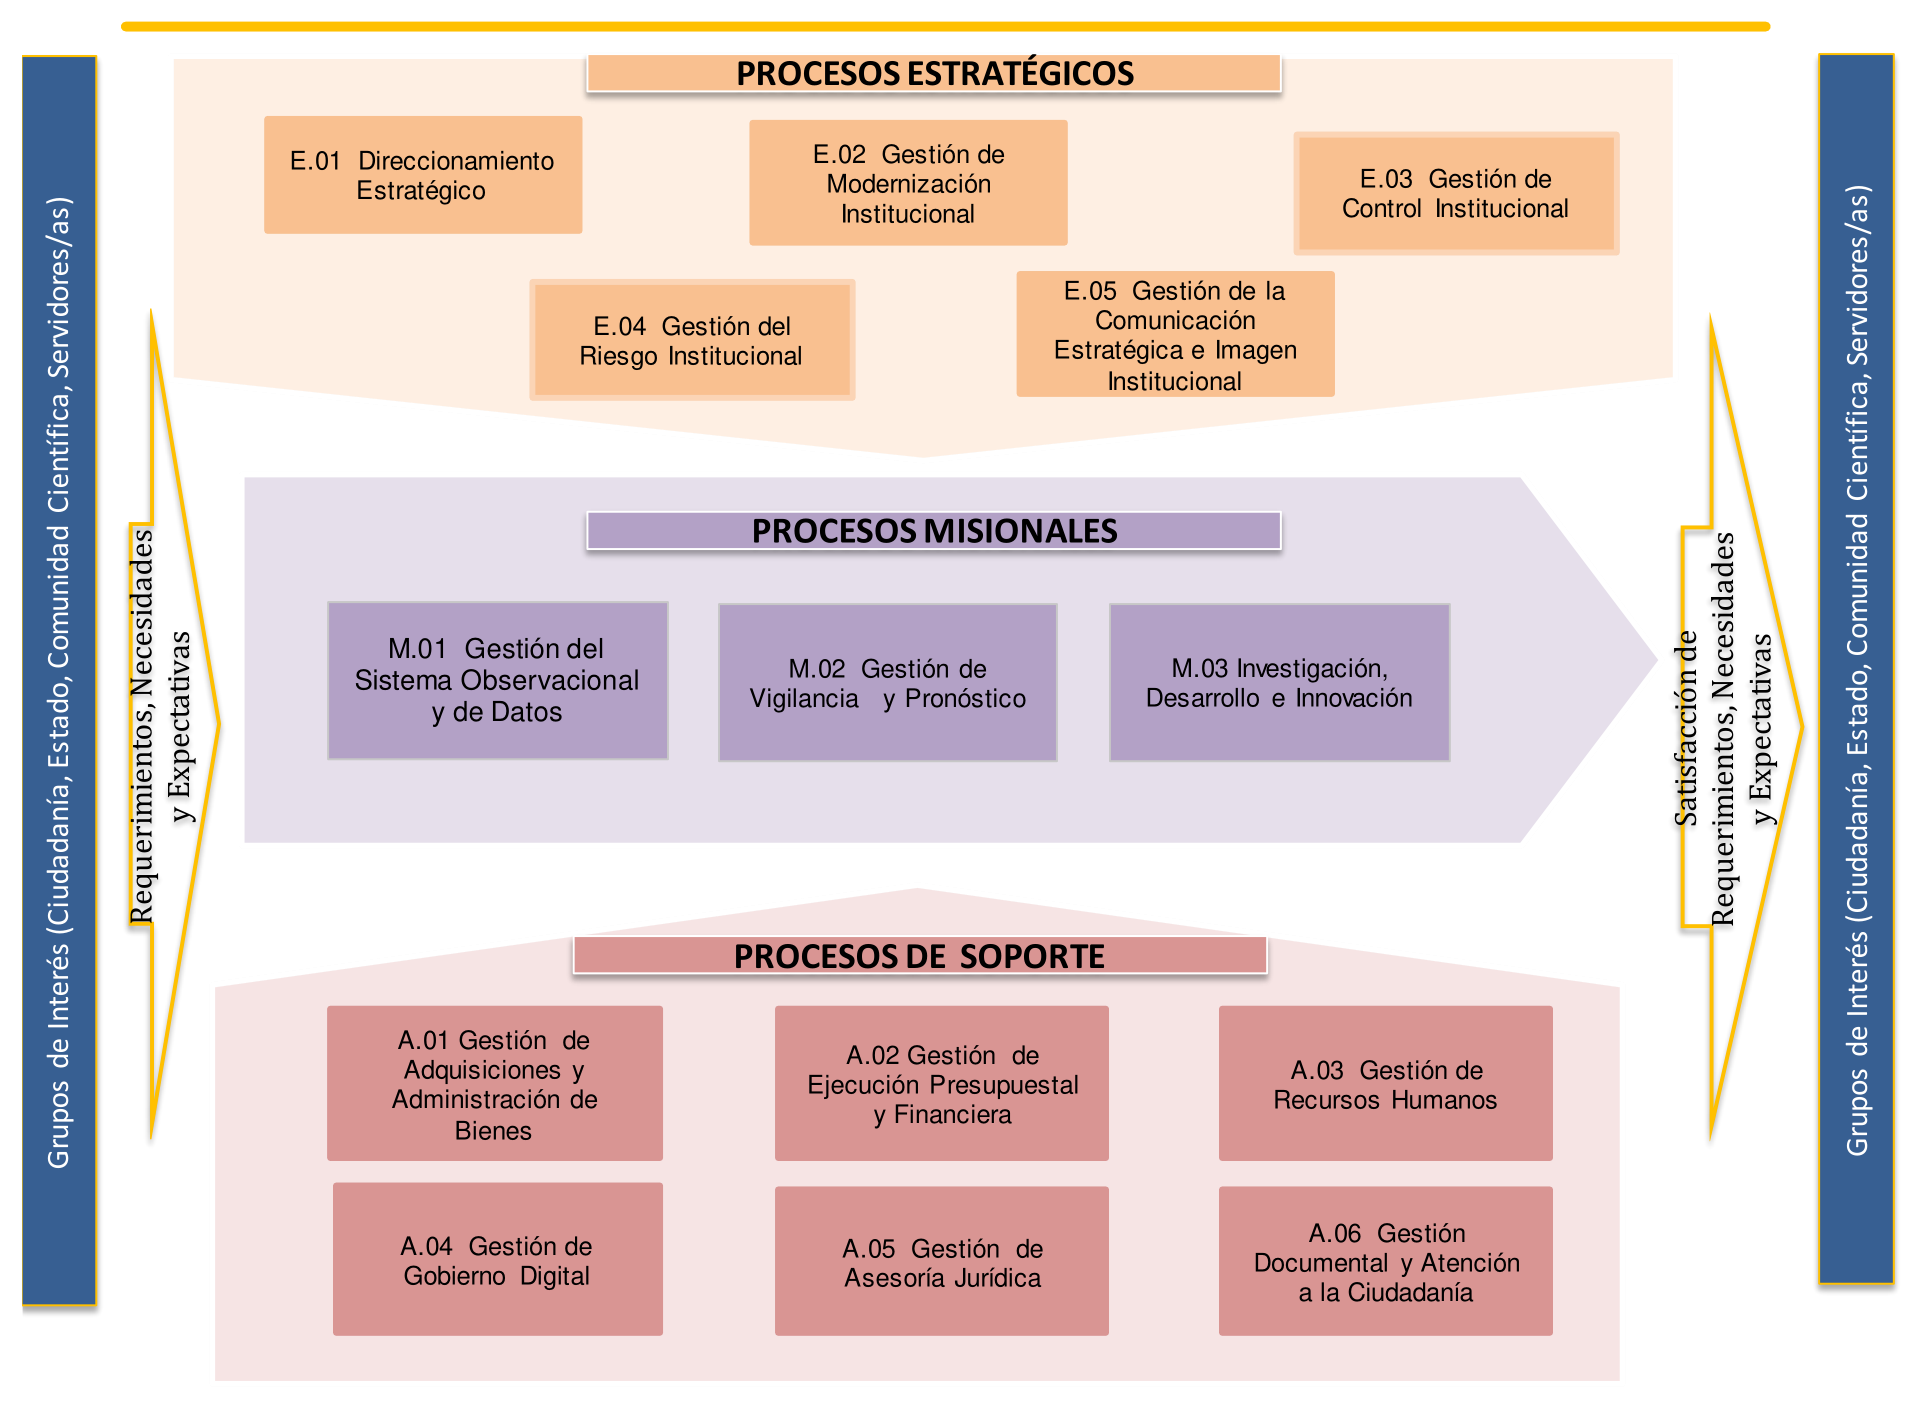
\includegraphics[height=8cm]{E_IMAGENES/2_MarcoTeorico/mapro}
  \caption{
    Mapa de Procesos del SENAMHI.\\
    Fuente: Manual de Procesos y Procedimientos 2020.
  }
  \label{fig:mapro}
\end{figure}

Según \cite{senamhi2020rof} entre sus funciones se encuentra ``Organizar, normar 
y promover un sistema de vigilancia del medio ambiente atmosférico del país, a 
fin de prevenir los peligros de la contaminación ambiental''. Esta función se 
materializa en el proceso misional 02 ``Gestión de Vigilancia y Pronóstico'' del 
Mapa de Procesos que se observa en la figura \ref{fig:mapro}.

\begin{figure}[H]
  \centering
  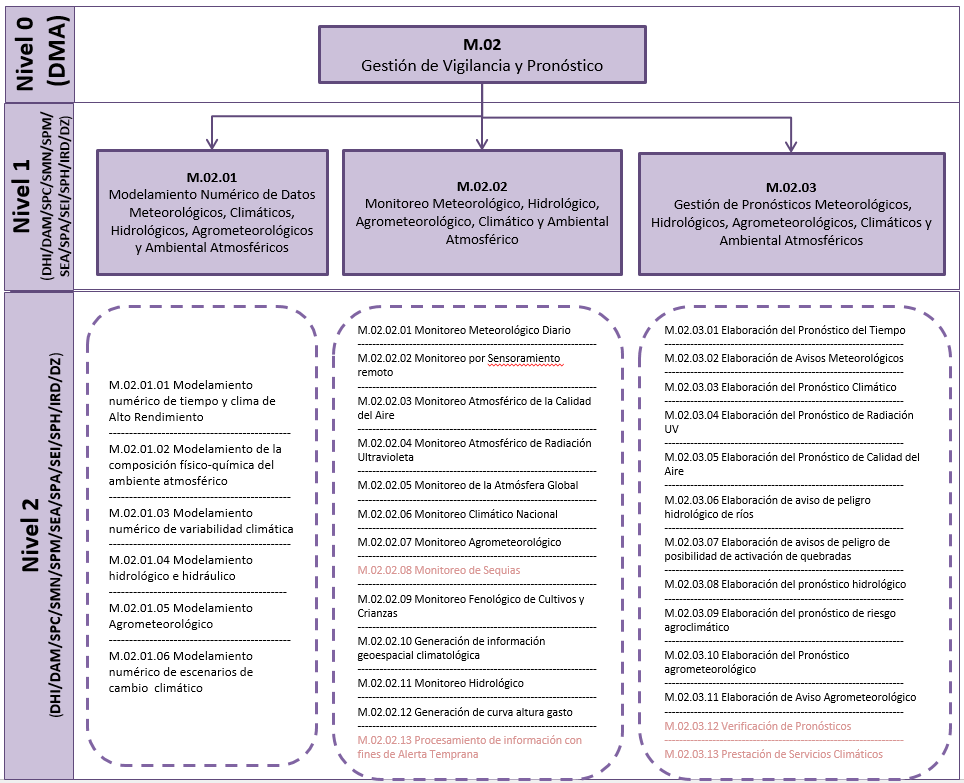
\includegraphics[height=8cm]{E_IMAGENES/2_MarcoTeorico/PM02}
  \caption{
    Proceso misional 02: Gestión de vigilancia y pronóstico\\
    Fuente: Manual de Procesos y Procedimientos 2020.
  }
  \label{fig:pm02}
\end{figure}

El proceso M.02.03, ``Gestión de Pronósticos Meteorológicos, Hidrológicos, 
Agrometeorológicos, Climáticos y Ambiental Atmosféricos'', que se observa en la 
figura \ref{fig:pm02} comprende entre sus procedimientos la elaboración de 
pronósticos del tiempo y tiene como uno de sus productos el pronóstico a muy 
corto plazo. 

De acuerdo a \cite{senamhi2021govdig}, es parte del Plan de Gobierno Digital del 
SENAMHI la ampliación de funcionalidades del sistema de pronóstico inmediato 
(nowcasting).
